%%%%%%%%%%%%%%%%%%%%%%%%%%%%%%%%%%%%%%%%%
% Arsclassica Article
% LaTeX Template
% Version 1.1 (10/6/14)
%
% This template has been downloaded from:
% http://www.LaTeXTemplates.com
%
% Original author:
% Lorenzo Pantieri (http://www.lorenzopantieri.net) with extensive modifications by:
% Vel (vel@latextemplates.com)
%
% License:
% CC BY-NC-SA 3.0 (http://creativecommons.org/licenses/by-nc-sa/3.0/)
%
%%%%%%%%%%%%%%%%%%%%%%%%%%%%%%%%%%%%%%%%%

%----------------------------------------------------------------------------------------
%	PACKAGES AND OTHER DOCUMENT CONFIGURATIONS
%----------------------------------------------------------------------------------------

\documentclass[
10pt, % Main document font size
a4paper, % Paper type, use 'letterpaper' for US Letter paper
oneside, % One page layout (no page indentation)
%twoside, % Two page layout (page indentation for binding and different headers)
headinclude,footinclude, % Extra spacing for the header and footer
BCOR5mm, % Binding correction
]{scrartcl}

%%%%%%%%%%%%%%%%%%%%%%%%%%%%%%%%%%%%%%%%%
% Arsclassica Article
% Structure Specification File
%
% This file has been downloaded from:
% http://www.LaTeXTemplates.com
%
% Original author:
% Lorenzo Pantieri (http://www.lorenzopantieri.net) with extensive modifications by:
% Vel (vel@latextemplates.com)
%
% License:
% CC BY-NC-SA 3.0 (http://creativecommons.org/licenses/by-nc-sa/3.0/)
%
%%%%%%%%%%%%%%%%%%%%%%%%%%%%%%%%%%%%%%%%%

%----------------------------------------------------------------------------------------
%	REQUIRED PACKAGES
%----------------------------------------------------------------------------------------

\usepackage[
nochapters, % Turn off chapters since this is an article        
beramono, % Use the Bera Mono font for monospaced text (\texttt)
eulermath,% Use the Euler font for mathematics
pdfspacing, % Makes use of pdftex’ letter spacing capabilities via the microtype package
dottedtoc % Dotted lines leading to the page numbers in the table of contents
]{classicthesis} % The layout is based on the Classic Thesis style

\usepackage{arsclassica} % Modifies the Classic Thesis package

\usepackage[T1]{fontenc} % Use 8-bit encoding that has 256 glyphs

\usepackage[utf8]{inputenc} % Required for including letters with accents

\usepackage{graphicx} % Required for including images
\graphicspath{{Figures/}} % Set the default folder for images

\usepackage{enumitem} % Required for manipulating the whitespace between and within lists

\usepackage{lipsum} % Used for inserting dummy 'Lorem ipsum' text into the template

\usepackage{subfig} % Required for creating figures with multiple parts (subfigures)

\usepackage{amsmath,amssymb,amsthm} % For including math equations, theorems, symbols, etc

\usepackage{varioref} % More descriptive referencing

%----------------------------------------------------------------------------------------
%	THEOREM STYLES
%---------------------------------------------------------------------------------------

\theoremstyle{definition} % Define theorem styles here based on the definition style (used for definitions and examples)
\newtheorem{definition}{Definition}

\theoremstyle{plain} % Define theorem styles here based on the plain style (used for theorems, lemmas, propositions)
\newtheorem{theorem}{Theorem}

\theoremstyle{remark} % Define theorem styles here based on the remark style (used for remarks and notes)

%----------------------------------------------------------------------------------------
%	HYPERLINKS
%---------------------------------------------------------------------------------------

\hypersetup{
%draft, % Uncomment to remove all links (useful for printing in black and white)
colorlinks=true, breaklinks=true, bookmarks=true,bookmarksnumbered,
urlcolor=webbrown, linkcolor=RoyalBlue, citecolor=webgreen, % Link colors
pdftitle={}, % PDF title
pdfauthor={\textcopyright}, % PDF Author
pdfsubject={}, % PDF Subject
pdfkeywords={}, % PDF Keywords
pdfcreator={pdfLaTeX}, % PDF Creator
pdfproducer={LaTeX with hyperref and ClassicThesis} % PDF producer
} % Include the structure.tex file which specified the document structure and layout

\usepackage[italian]{babel}

\hyphenation{Fortran hy-phen-ation} % Specify custom hyphenation points in words with dashes where you would like hyphenation to occur, or alternatively, don't put any dashes in a word to stop hyphenation altogether

%----------------------------------------------------------------------------------------
%	TITLE AND AUTHOR(S)
%----------------------------------------------------------------------------------------

\title{\normalfont\spacedallcaps{Analisi Stabilizzatore SIAI MARCHETTI SF-260}} % The article title

\author{\spacedlowsmallcaps{Claudio Caccia}} % The article author(s) - author affiliations need to be specified in the AUTHOR AFFILIATIONS block

\date{\today} % An optional date to appear under the author(s)

%----------------------------------------------------------------------------------------

\begin{document}

%----------------------------------------------------------------------------------------
%	HEADERS
%----------------------------------------------------------------------------------------

\renewcommand{\sectionmark}[1]{\markright{\spacedlowsmallcaps{#1}}} % The header for all pages (oneside) or for even pages (twoside)
%\renewcommand{\subsectionmark}[1]{\markright{\thesubsection~#1}} % Uncomment when using the twoside option - this modifies the header on odd pages
\lehead{\mbox{\llap{\small\thepage\kern1em\color{halfgray} \vline}\color{halfgray}\hspace{0.5em}\rightmark\hfil}} % The header style

\pagestyle{scrheadings} % Enable the headers specified in this block

%----------------------------------------------------------------------------------------
%	TABLE OF CONTENTS & LISTS OF FIGURES AND TABLES
%----------------------------------------------------------------------------------------

\maketitle % Print the title/author/date block

\setcounter{tocdepth}{2} % Set the depth of the table of contents to show sections and subsections only

\tableofcontents % Print the table of contents

\listoffigures % Print the list of figures

\listoftables % Print the list of tables

%----------------------------------------------------------------------------------------
%	ABSTRACT
%----------------------------------------------------------------------------------------

\section*{Oggetto} % This section will not appear in the table of contents due to the star (\section*)

Scopo dell'analisi consiste nell'effettuare una modellazione ad elementi finiti dello stabilizzatore del velivolo \emph{SIAI Marchetti SF-260} (cfr. Figura \ref{fig:stab260}) nelle condizioni di carico specificate nella documentazione fornita, arrivando a determinare la configurazione deformata (freccia massima, angolo di torsione, etc.) ed una stima dello stato di sforzo nella struttura.

\begin{figure}[tb]
	\centering 
	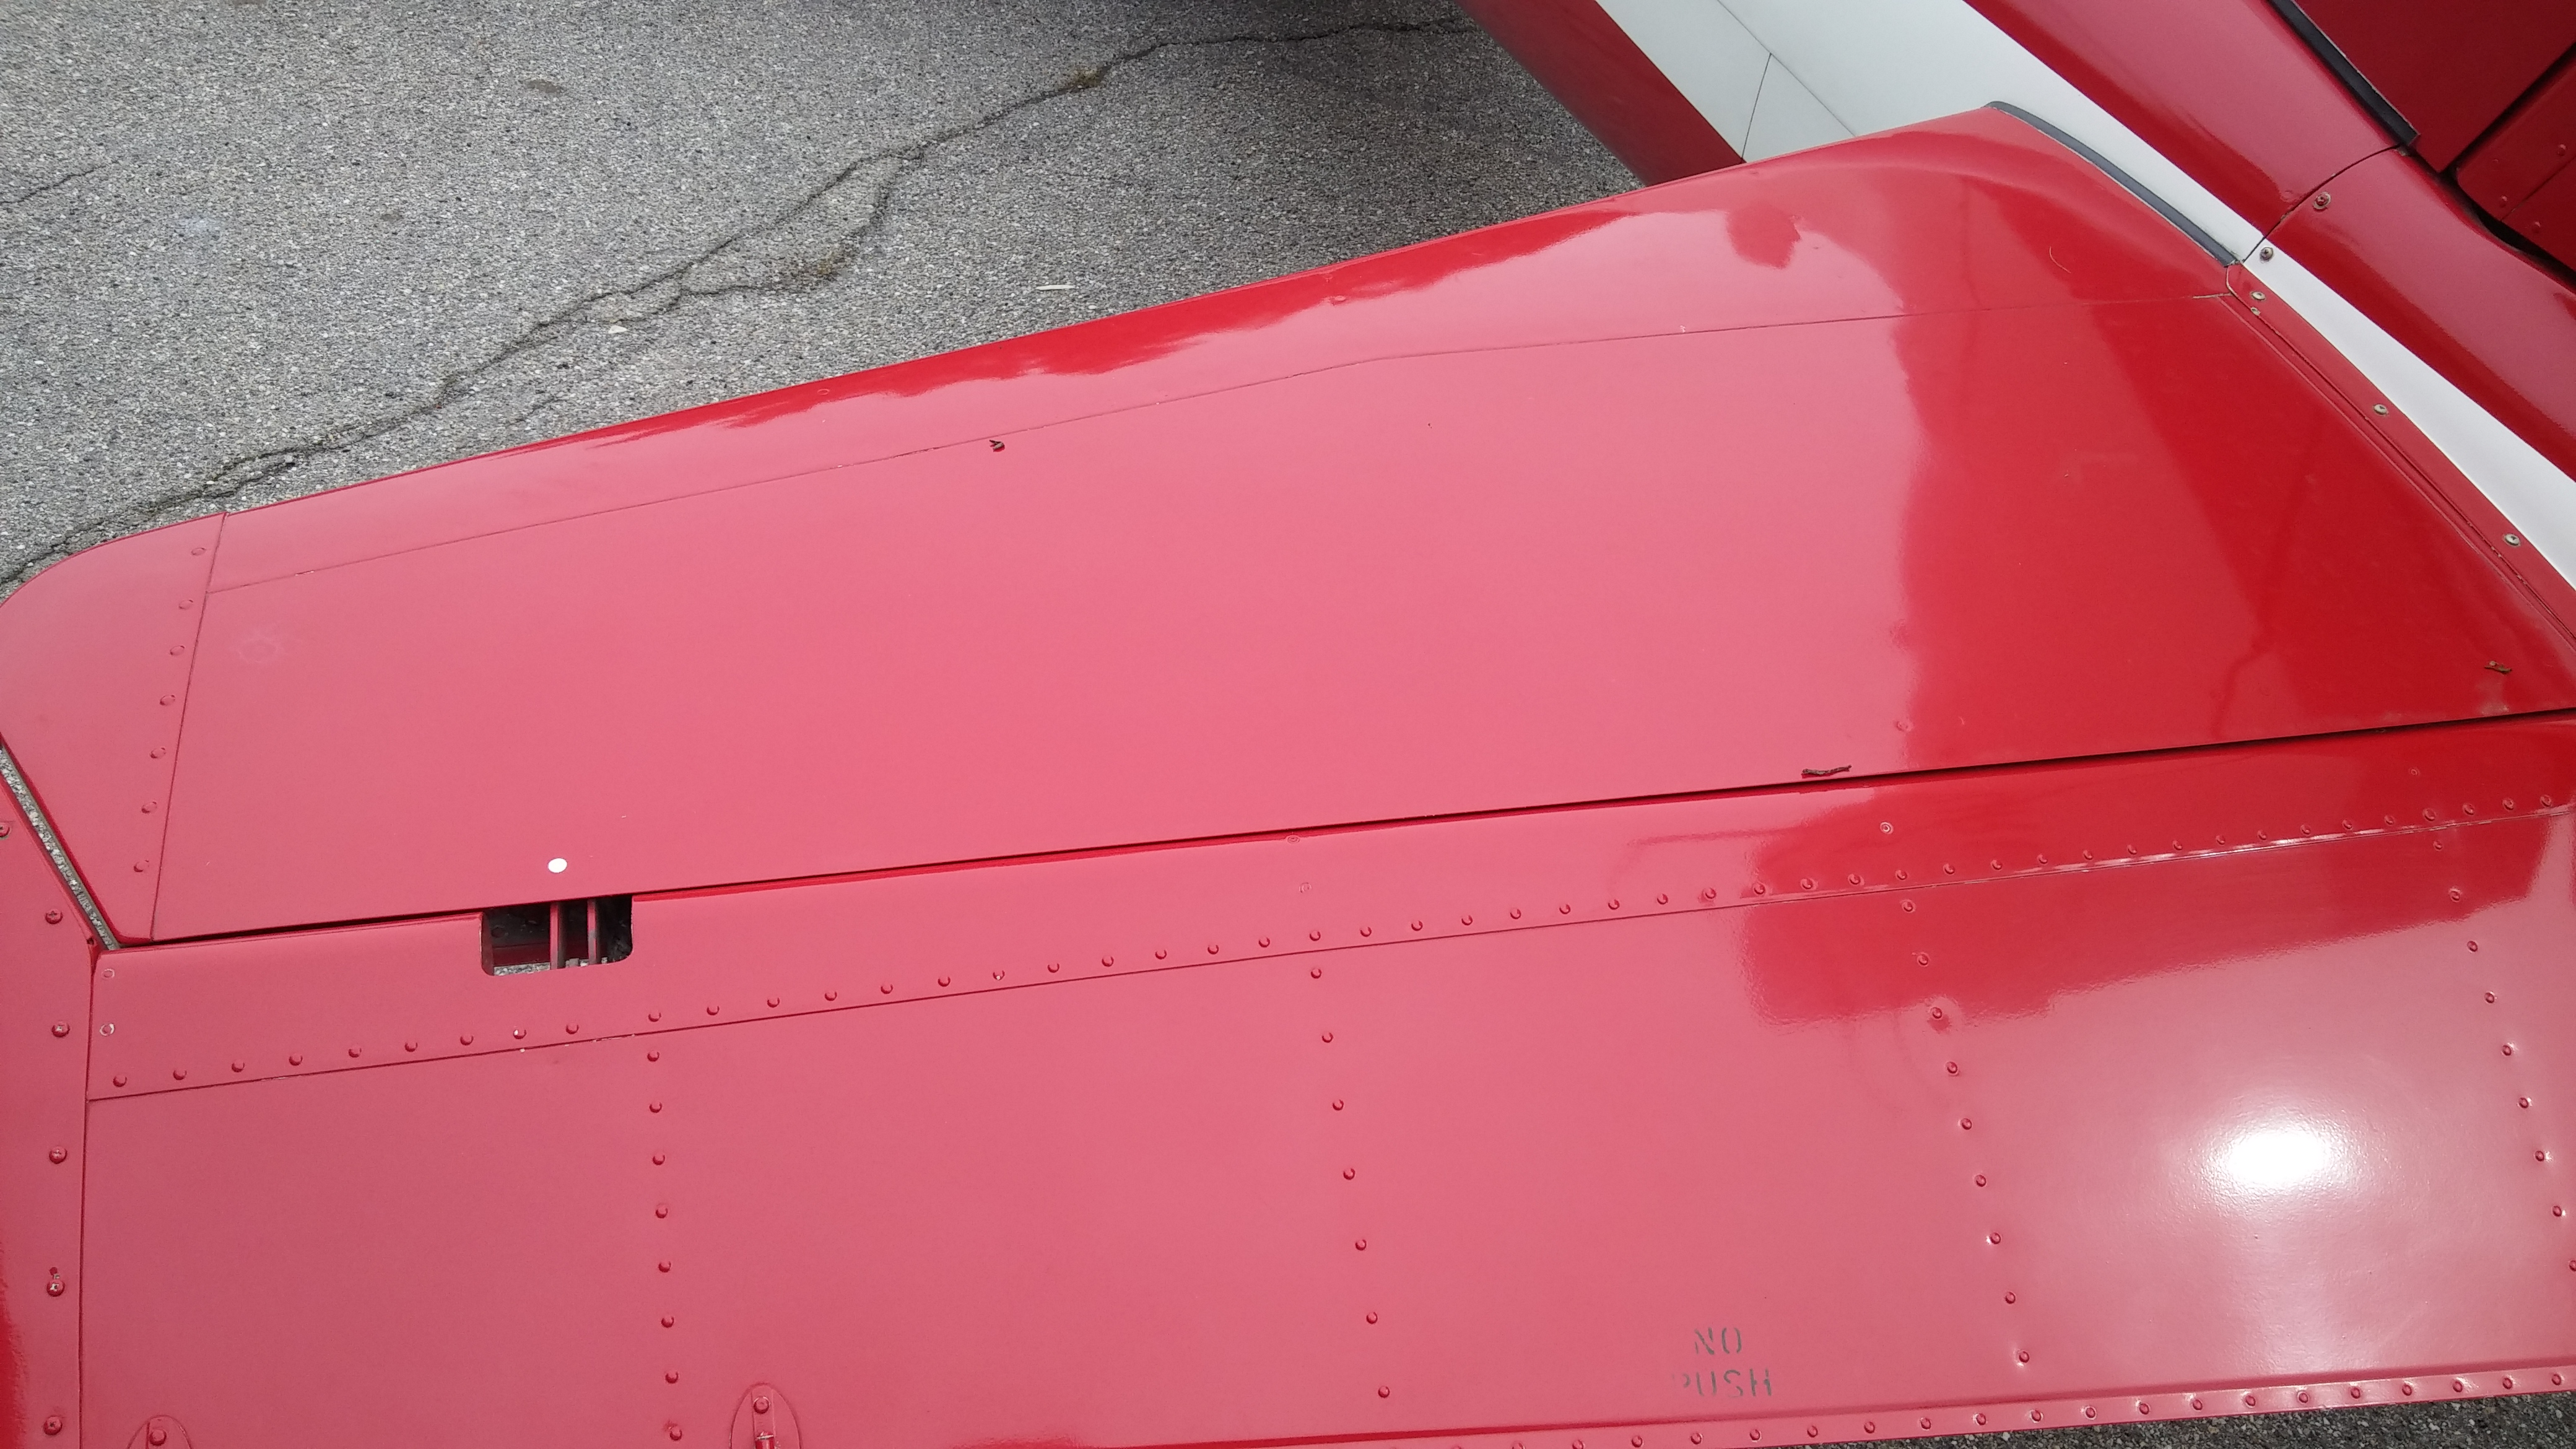
\includegraphics[width=0.9\columnwidth]{stab.jpg} 
	\caption[foto stabilizzatore]{Foto dello stabilizzatore} % The text in the square bracket is the caption for the list of figures while the text in the curly brackets is the figure caption
	\label{fig:stab260} 
\end{figure}

%\url{http://www.mcescher.com/}
%----------------------------------------------------------------------------------------
%	AUTHOR AFFILIATIONS
%----------------------------------------------------------------------------------------

%{\let\thefootnote\relax\footnotetext{* \textit{Department of Biology, University of Examples, London, United Kingdom}}}

%{\let\thefootnote\relax\footnotetext{\textsuperscript{1} \textit{Department of Chemistry, University of Examples, London, United Kingdom}}}

%----------------------------------------------------------------------------------------

\newpage % Start the article content on the second page, remove this if you have a longer abstract that goes onto the second page

%----------------------------------------------------------------------------------------
%	INTRODUCTION
%----------------------------------------------------------------------------------------

\section{Strumenti}

%A statement\footnote{Example of a footnote} requiring citation \cite{Figueredo:2009dg}.
%Some mathematics in the text: $\cos\pi=-1$ and $\alpha$.

L'analisi \emph{FEM} \`{e} stata eseguita utilizzando i seguenti sotfware di modellazione e calcolo:

\begin{itemize}
	\item \textbf{Code-Aster} \url{http://code-aster.org} (vers. 13.1) per la modellazione ad elementi finiti,
	\item \textbf{{Salome}} \url{http://www.salome-platform.org} (vers. 7.7.1) per modellazione geometrica e mesh
	\item \textbf{ParaView} \url{http://www.paraview.org}(vers. 4.7) per il post-processing
	\item \textbf{Python} per ogni attivit\`{a} di calcolo
\end{itemize}

Il codice scritto per la realizzazione delle analisi \`{e} disponibile al seguente indirizzo: \url{https://github.com/Ccaccia73/SF206_stab_analysis}



\section{Panoramica delle analisi}

Lo studio comprende:

\begin{itemize}
	\item Unit\`{a} di misura: \textbf{SI} [N, mm, t]
	\item Numero di geometrie: \textbf{1}
	\item Numero di mesh: \textbf{3}
	\item Numero di analisi FEM: \textbf{6}
\end{itemize}

Ad esse si aggiungono alcune analisi complementari per la verifica e l'ottimizzazione degli elementi ed ulteriori calcoli per la verifica della validit\`{a} delle analisi compiute.


\section{Geometria}

Le parti della geometria sono rappresentate in Figura \ref{fig:geom}, da cui sono stati soppressi i pannelli superiori per rendere visibili gli elementi:

\begin{itemize}
	\item Longherone principale (blu)
	\item Longherone anteriore (verde)
	\item Centine (grigio)
	\item Pannelli posteriori (rosso)
	\item Pannelli anteriori (giallo)
\end{itemize}

Il sistema di riferimento è illustrato in figura: l'origine è in mezzeria a metà longherone, lo stabilizzatore è diretto lungo \emph{z}, l'asse \emph{x} è diretto verso la coda e \emph{y} verso l'alto.

\begin{figure}[tb]
	\centering 
	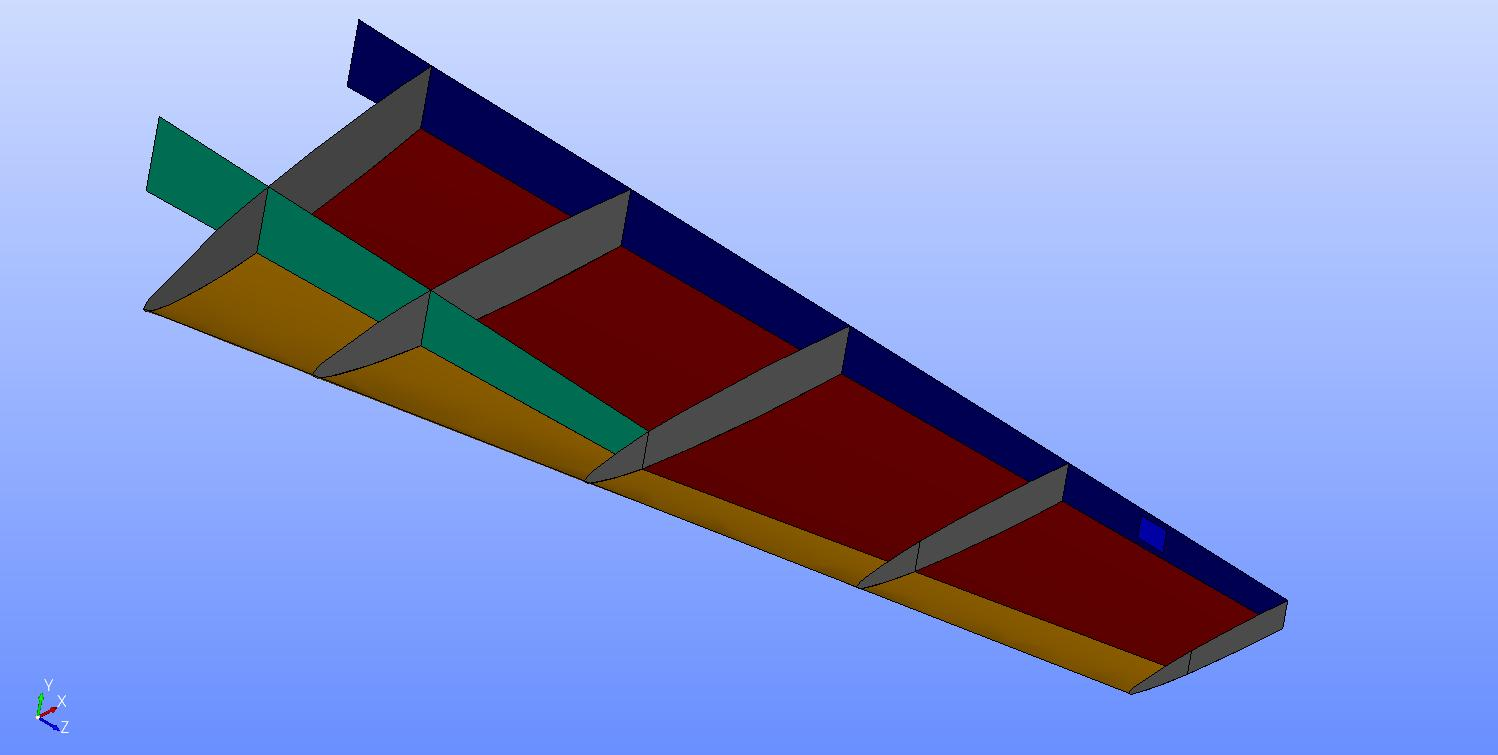
\includegraphics[width=0.9\columnwidth]{geom.jpg} 
	\caption[Geometria stabilizzatore]{Geometria stab. SF260} % The text in the square bracket is the caption for the list of figures while the text in the curly brackets is the figure caption
	\label{fig:geom} 
\end{figure}


\section{Caratterizzazione degli elementi}

Prima di procedere all'analisi è necessario caratterizzare opportunamente le componenti dello stabilizzatore, con l'intento di semplificare la struttura il più possibile senza perdere significatività. 

\subsection{Centine}

La struttura delle 5 centine è composta da un'anima spessa 0.64mm e due flange lunghe 15mm. La numerazione parte dalla mezzeria. Le prime 4 centine sono caratterizzate da fori di alleggerimento.
Per semplificare il modello si è scelto di modellare la centina con le seguenti caratteristiche:

\begin{itemize}
	\item Sono stati trascurati i fori di alleggerimento,
	\item l'anima è stata modellata con elementi di tipo \emph{plate},
	\item le flange sono state modellate con elementi di tipo \emph{beam}.
\end{itemize} 

In questo modo si rischia di perdere informazioni relative ad eventuali concentrazioni di sforzo in corrispondenza dei fori, inoltre la rigidezza flesso-torsionale della centina viene leggermente modificata.\\
Per ovviare a questi inconvenienti sono state condotte analisi preliminari sulle centine al fine di:

\begin{itemize}
	\item definire uno spessore equivalente che replichi la stessa rigidezza flessionale della centina (ritenuta l'aspetto più significativo),
	\item analizzare l'andamento degli sforzi nella centina in condizioni di carico semplici per avere un'indicazione su eventuali concentrazioni di sforzi.
\end{itemize}

Per ogni centina sono state condotte le seguenti analisi:

\begin{itemize}
	\item centina originale incastrata in corrispondenza del longherone principale, movimento lungo \emph{z} impedito e carico unitario in estremità lungo \emph{y} (cedevolezza flessionale),
	\item centina originale incastrata in corrispondenza del longherone principale e coppia unitaria in estremità diretta secondo \emph{x} (cedevolezza torsionale),
	\item centina semplificata caricata nello stesso modo per determinare lo spessore equivalente che garantisca la stessa cedevolezza flessionale, infine verifica della cedevolezza torsionale. 
\end{itemize}

Nelle figure \ref{fig:C1_comp} e \ref{fig:C1plot}  si riportano ad esempio i risultati ottenuti per la \emph{centina 1}.

\begin{figure}[htb]
	\centering
	\subfloat[Centina 1: deformazione flessionale]{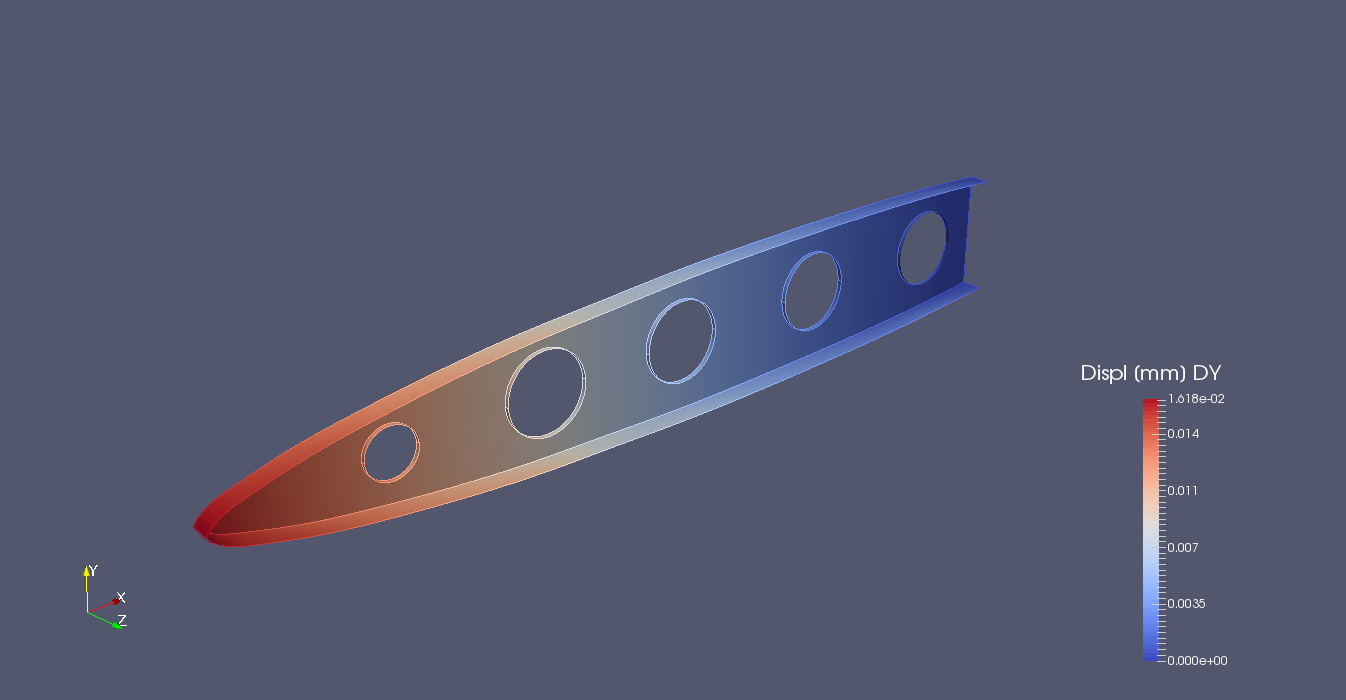
\includegraphics[width=.90\columnwidth]{C1_comp_DY.png}\label{fig:C1_DY}} \\
	\subfloat[Centina 1: VM stress]{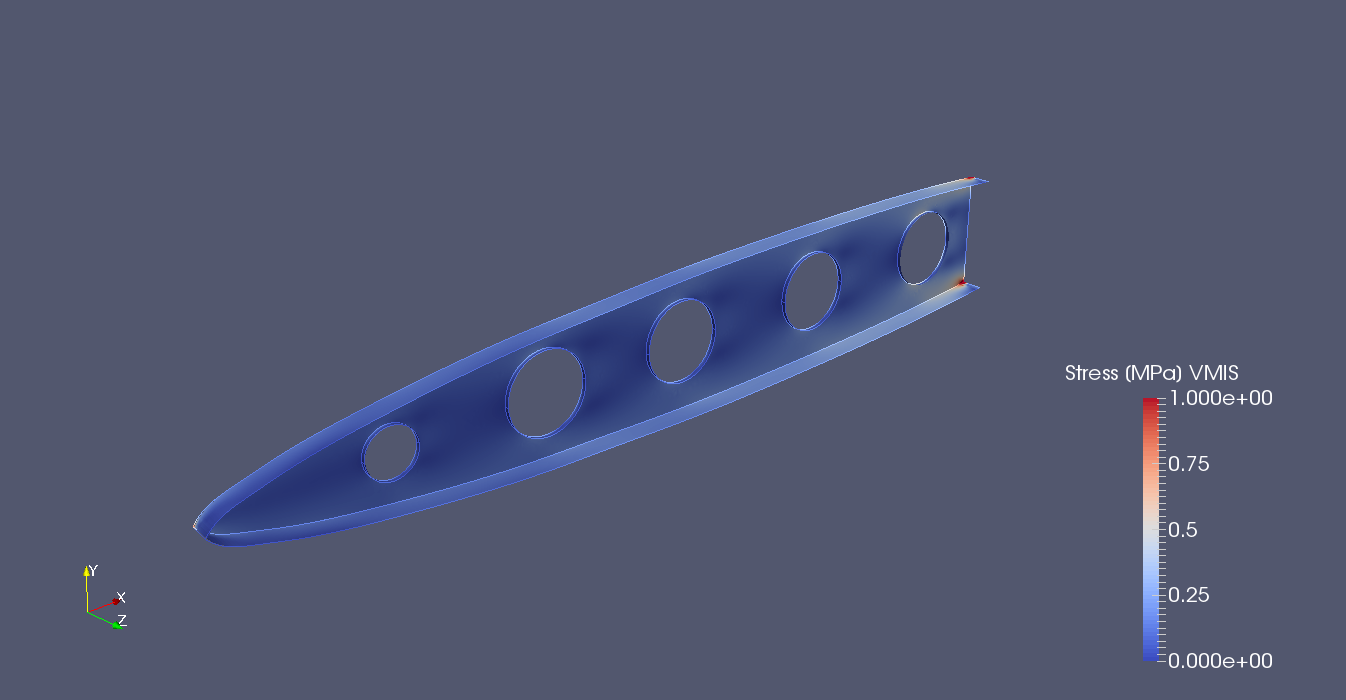
\includegraphics[width=.90\columnwidth]{C1_comp_VMIS.png}\label{fig:C1_VM}} \\
	\caption[Centina 1 completa]{Analisi Centina 1 completa} % The text in the square bracket is the caption for the list of figures while the text in the curly brackets is the figure caption
	\label{fig:C1_comp}
\end{figure}

\begin{figure}[htb]
	\centering
	\subfloat[Centina 1: VM stress root]{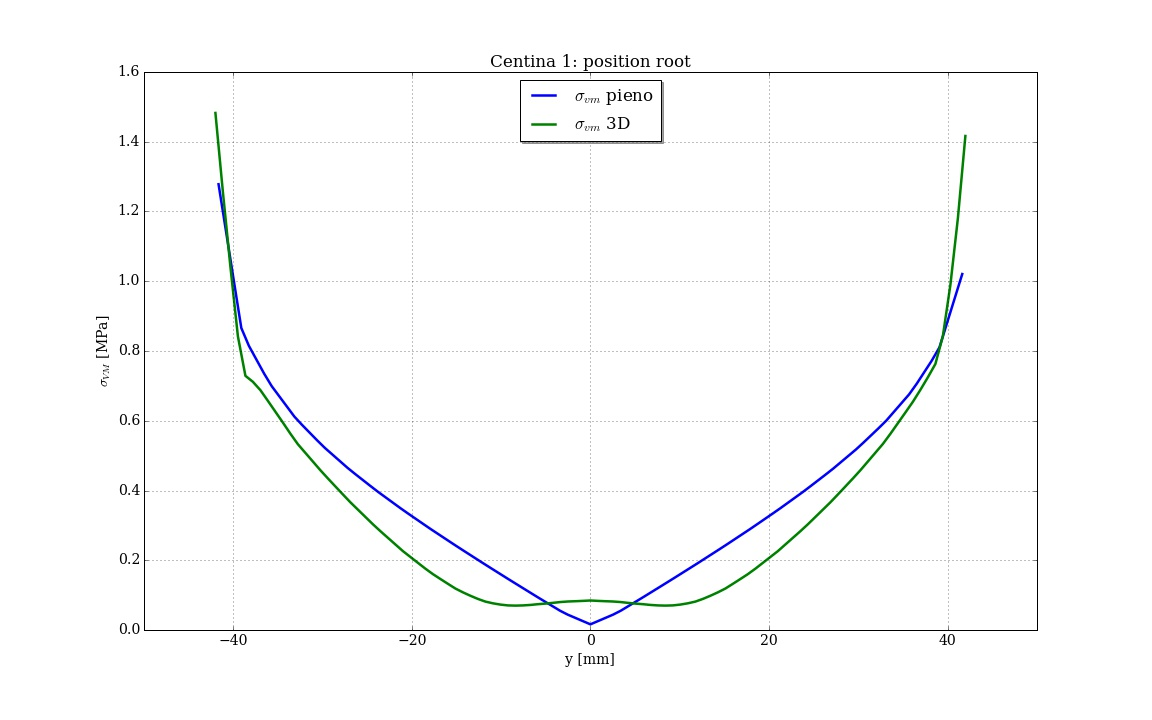
\includegraphics[width=.90\columnwidth]{C1_VM_root}\label{fig:C1_root}} \\
	\subfloat[Centina 1: VM stress @53.5mm]{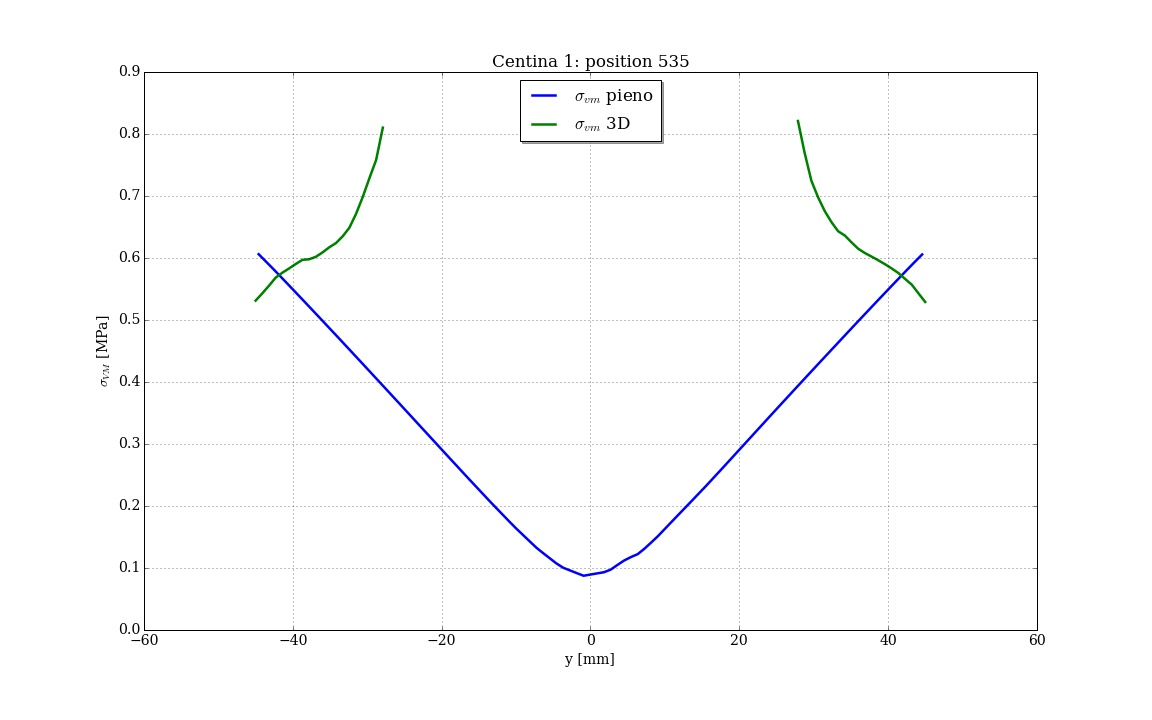
\includegraphics[width=.90\columnwidth]{C1_VM_535}\label{fig:C1_535}} \\
	\caption[Centina 1 confronto VM stress]{Centina 1 confronto VM stress} % The text in the square bracket is the caption for the list of figures while the text in the curly brackets is the figure caption
	\label{fig:C1plot}
\end{figure}

La figura \ref{fig:C1plot} fornisce un'indicazione sull'incremento degli sforzi nella centina (all'incastro ed in corrispondenza del primo foro, a $53.5mm$ dall'incastro) per effetto della presenza dei fori.


\begin{table}[hbt]
	\caption{Risultati delle analisi sulle centina}
	\centering
	\begin{tabular}{rcccccc}
		\toprule
		& \multicolumn{3}{c}{Completo} & \multicolumn{3}{c}{Semplificato}\\
		\cmidrule(r){2-4} \cmidrule(l){5-7} 
		& DY  & DRX & massa & spessore & DRX  & massa \\
		& $[\mu m/N]$ & $[\mu rad/Nmm]$ & $[g]$ & $[\mu m]$ & $[\mu rad/Nmm]$ & $[g]$ \\
		\midrule
		C1 & $16.18$ & $771$ & $105$ & $513$ & $458$ & $95$ \\
		C2 & $16.52$ & $782$ & $84$ & $497$ & $488$ & $75$ \\
		C3 & $14.10$ & $880$ & $67$ & $550$ & $372$ & $60$ \\
		C4 & $13.68$ & $841$ & $45$ & $526$ & $386$ & $39$ \\
		C5 & $13.26$ & $849$ & $29$ & $508$ & $356$ & $23$ \\
		\bottomrule
	\end{tabular}
	\label{tab:centine}
\end{table}

La tabella \ref{tab:centine} mostra come, a parità di rigidezza flessionale, le centine semplificate risultino più rigide torsionalmente e di poco più leggere. Si ritiene la semplificazione comunque accettabile e si utilizzano tali valori nell'analisi.

\newpage

\subsection{Longherone anteriore}

Il longherone anteriore (LA) è lungo $740mm$, ha uno spessore di $1.6mm$ ed è disposto dalla mezzeria fino alla centina 3. Come le centine ha una struttura a \textquotedblleft C\textquotedblright con fori di alleggerimento e un irrigidimento nella parte centrale.
Si operano semplificazioni simili a quelle adottate per le centine:

\begin{itemize}
	\item Modellizzazione dell'anima a \emph{plate} e delle flange a \emph{beam}
	\item eliminazione dei fori e determinazione di uno spessore equivalente
\end{itemize}

Nelle figure \ref{fig:FS_compl} e \ref{fig:FS_simp} si riportano i risultati ottenuti.


\begin{figure}[htb]
	\centering
	\subfloat[LA: sforzi ed azioni]{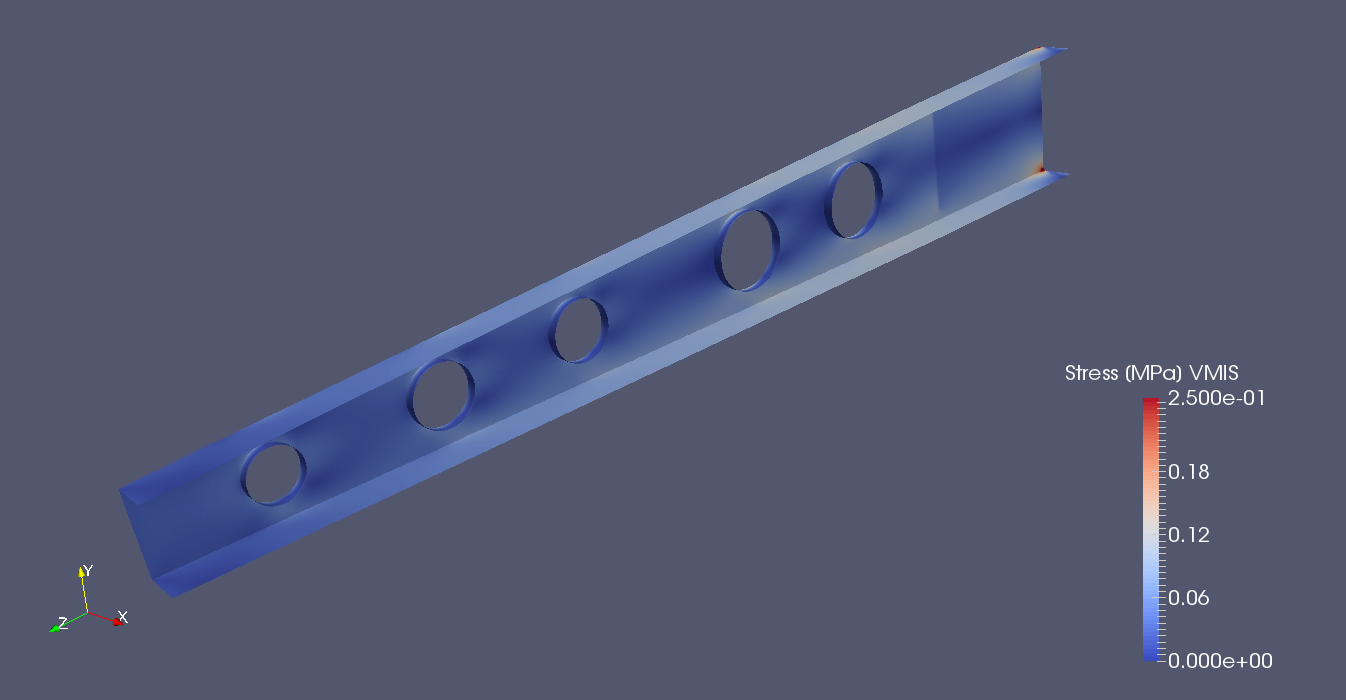
\includegraphics[width=.90\columnwidth]{FS_compl_VM.png}\label{fig:FSc_VM}} \\
	\subfloat[LA: deformazione]{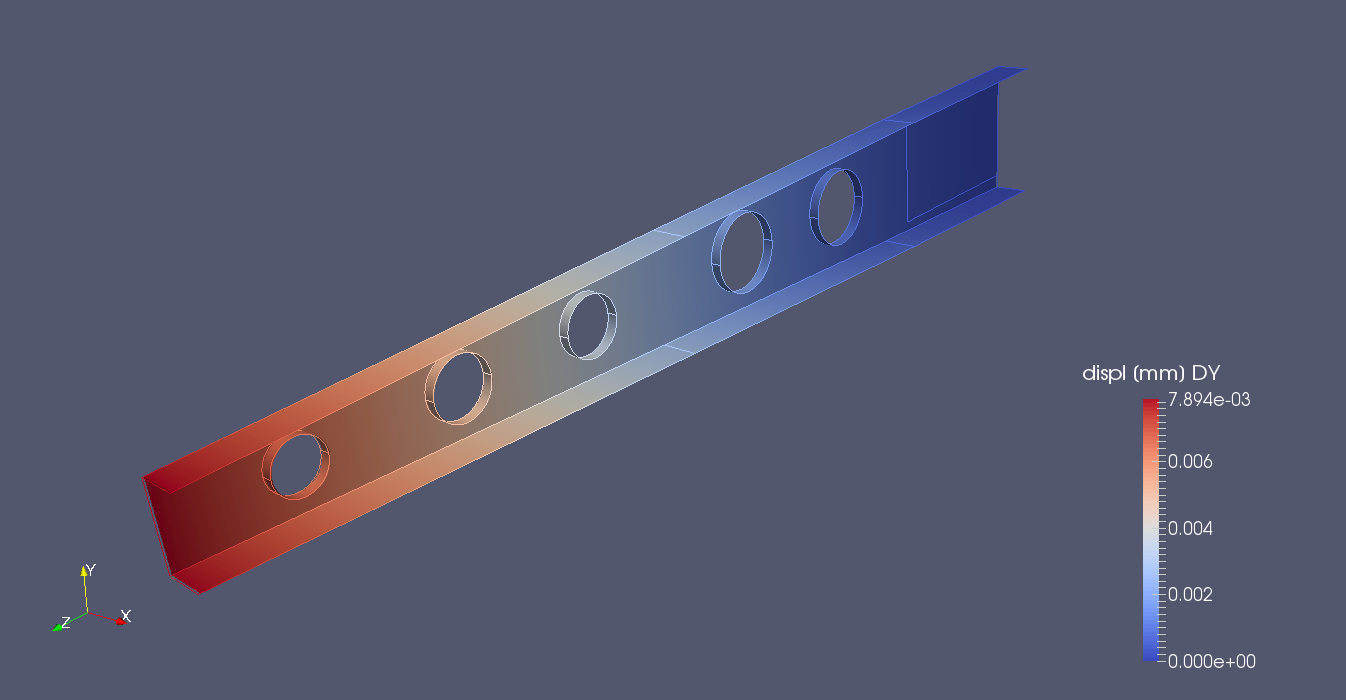
\includegraphics[width=.90\columnwidth]{FS_compl_DY.png}\label{fig:FSc_DY}} \\
	\caption[Longherone anteriore completo]{Analisi longherone anteriore completo} % The text in the square bracket is the caption for the list of figures while the text in the curly brackets is the figure caption
	\label{fig:FS_compl}
\end{figure}


\begin{figure}[htb]
	\centering
	\subfloat[LA: sforzi ed azioni]{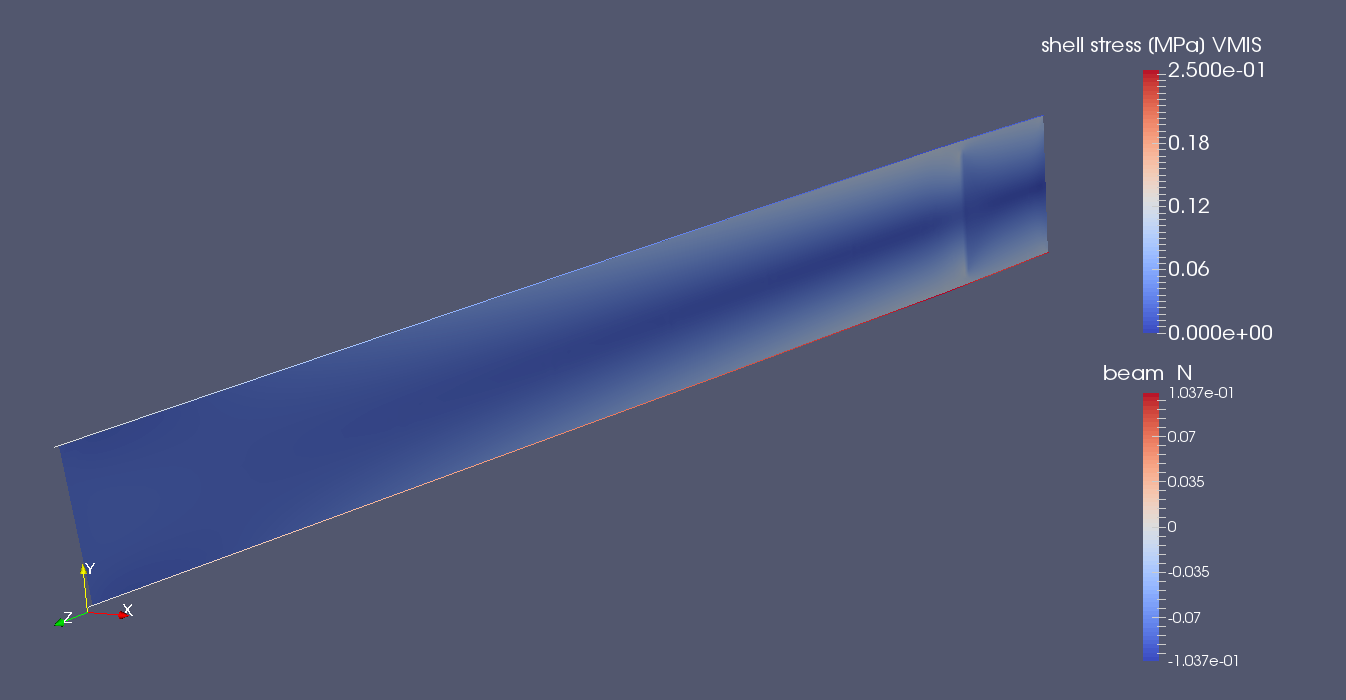
\includegraphics[width=.90\columnwidth]{FS_simp_str.png}\label{fig:FSs_VM}} \\
	\subfloat[LA: deformazione]{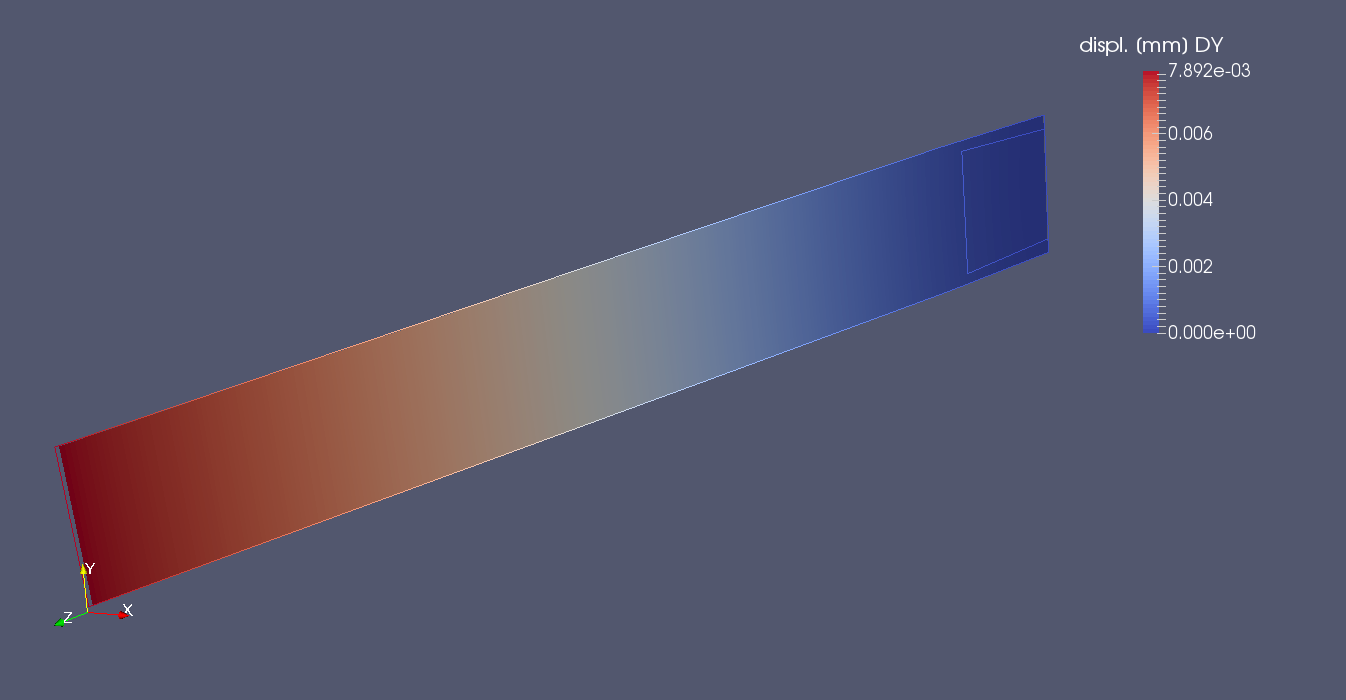
\includegraphics[width=.90\columnwidth]{FS_simp_DY.png}\label{fig:FSs_DY}} \\
	\caption[Longherone anteriore semplificato]{Analisi longherone anteriore semplificato} % The text in the square bracket is the caption for the list of figures while the text in the curly brackets is the figure caption
	\label{fig:FS_simp}
\end{figure}

Il calcolo teorico di una mensola incastrata linearmente rastremata con le stesse dimensioni del longherone anteriore fornisce una cedevolezza flessionale di $8\cdot10^{-3} mm/N$ contro i $7.89\cdot10^{-3} mm/N$ del modello, confermando la validità della simulazione.\\
La tabella \ref{tab:FS} riporta la sintesi dei risultati ottenuti.

\begin{table}[hbt]
	\caption{Risultati delle analisi sul longherone anteriore}
	\centering
	\begin{tabular}{rcccccc}
		\toprule
		& \multicolumn{3}{c}{Completo} & \multicolumn{3}{c}{Semplificato}\\
		\cmidrule(r){2-4} \cmidrule(l){5-7} 
		& DY  & DRZ & massa & spessore & DRZ  & massa \\
		& $[\mu m/N]$ & $[\mu rad/Nmm]$ & $[g]$ & $[mm]$ & $[\mu rad/Nmm]$ & $[g]$ \\
		\midrule
		LA & $7.89$ & $114$ & $454$ & $1.471$ & $128$ & $429$ \\
		\bottomrule
	\end{tabular}
	\label{tab:FS}
\end{table}


\subsection{Longherone principale}

Il longherone principale (LP) è privo di fori di alleggerimento, ha degli irrigidimenti in corrispondenza della zona centrale e tra le centine 4 e 5, inoltre ha un corrente a \textquotedblleft U\textquotedblright \ per tutta la lunghezza ed un corrente a \textquotedblleft L\textquotedblright fino alla distanza di $510mm$. \`{E} stato modellato direttamente nel sistema completo, con le seguenti caratteristiche:

\begin{itemize}
	\item spessori (elementi di tipo \emph{plate}) nelle 5 sezioni del LP:
	\begin{itemize}
		\item $1.6+2mm$ nella sezione 1, tenendo condo in modo semplificato dell'irrigidimento
		\item $1.6mm$ nelle sezioni 2,3 e 4
		\item $1.6+2.9mm$ nella sezione 5, tenendo conto dell'irrigidimento
	\end{itemize}
	\item elementi di tipo \emph{beam}:
	\begin{itemize}
		\item corrente a \textquotedblleft U\textquotedblright \ più corrente a \textquotedblleft L\textquotedblright nelle sezioni 1 e 2, tenendo conto in modo semplificato del corrente a \textquotedblleft L\textquotedblright, più lungo e rastremato
		\item corrente a \textquotedblleft U\textquotedblright \ nelle sezioni 3 e 4
		\item corrente a \textquotedblleft U\textquotedblright \ più flangia da $2.9 \times 25 mm$ nella sezione 5
	\end{itemize}
\end{itemize}


\subsection{Correnti}

Oltre ai correnti nel longherone principale sono presenti dei correnti a \textquotedblleft L\textquotedblright \ nelle sezioni 4 e 5, oltre il longherone principale. Vengono modellati con elementi di tipo \emph{beam}.

\subsection{Pannelli}

Tutti i pannelli vengono modellati con elementi di tipo \emph{plate}, spessi $0.64mm$ nella parte anteriore (fino al LA o ai correnti) e $0.81mm$ nella parte posteriore. 


\newpage

\section{Mesh}

La mesh è stata generata elemento per elemento, realizzando poi un'unica \emph{compound mesh} e verificando che gli elementi (nodi e spigoli) fossero coincidenti.
La mesh è composta da 7271 elementi di cui:

\begin{itemize}
	\item $7138$ elementi di tipo \emph{QUAD4}
	\item $133$ elementi di tipo \emph{TRIA3}
\end{itemize} 

\begin{figure}[htb]
	\centering
	\subfloat[mesh: pannelli]{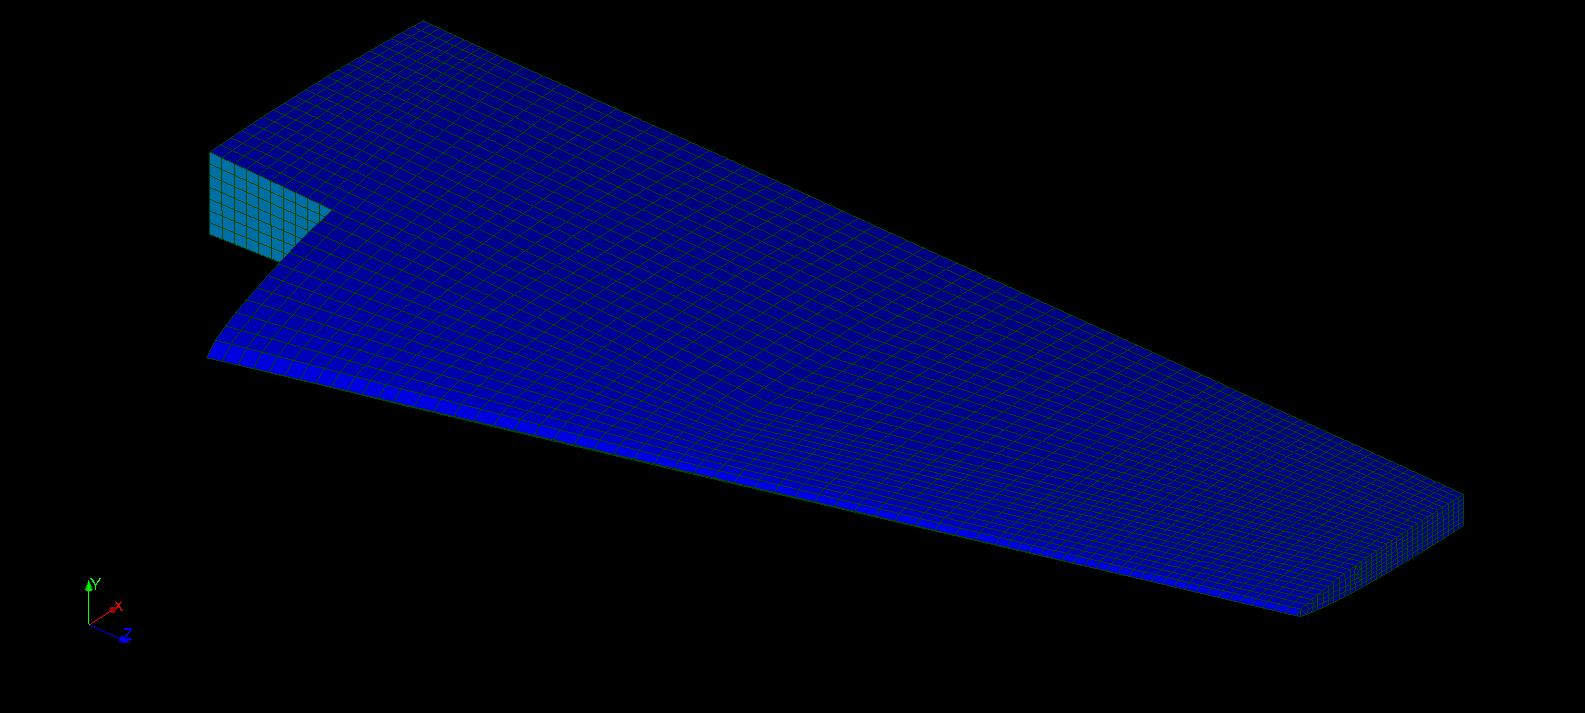
\includegraphics[width=.90\columnwidth]{mesh1.jpg}\label{fig:mesh1}} \\
	\subfloat[mesh: centine e longheroni]{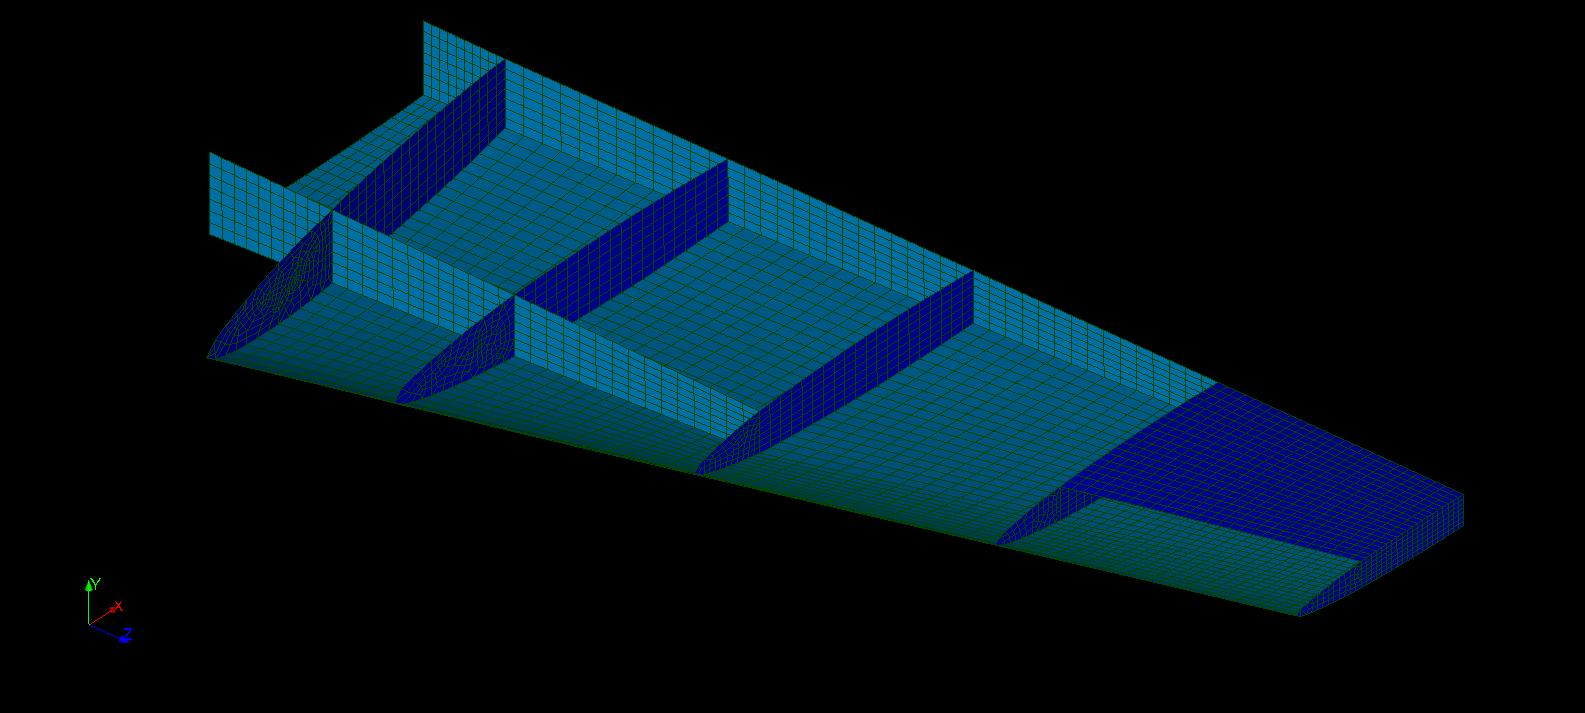
\includegraphics[width=.90\columnwidth]{mesh2.jpg}\label{fig:mesh2}} \\
	\subfloat[mesh: elementi beam]{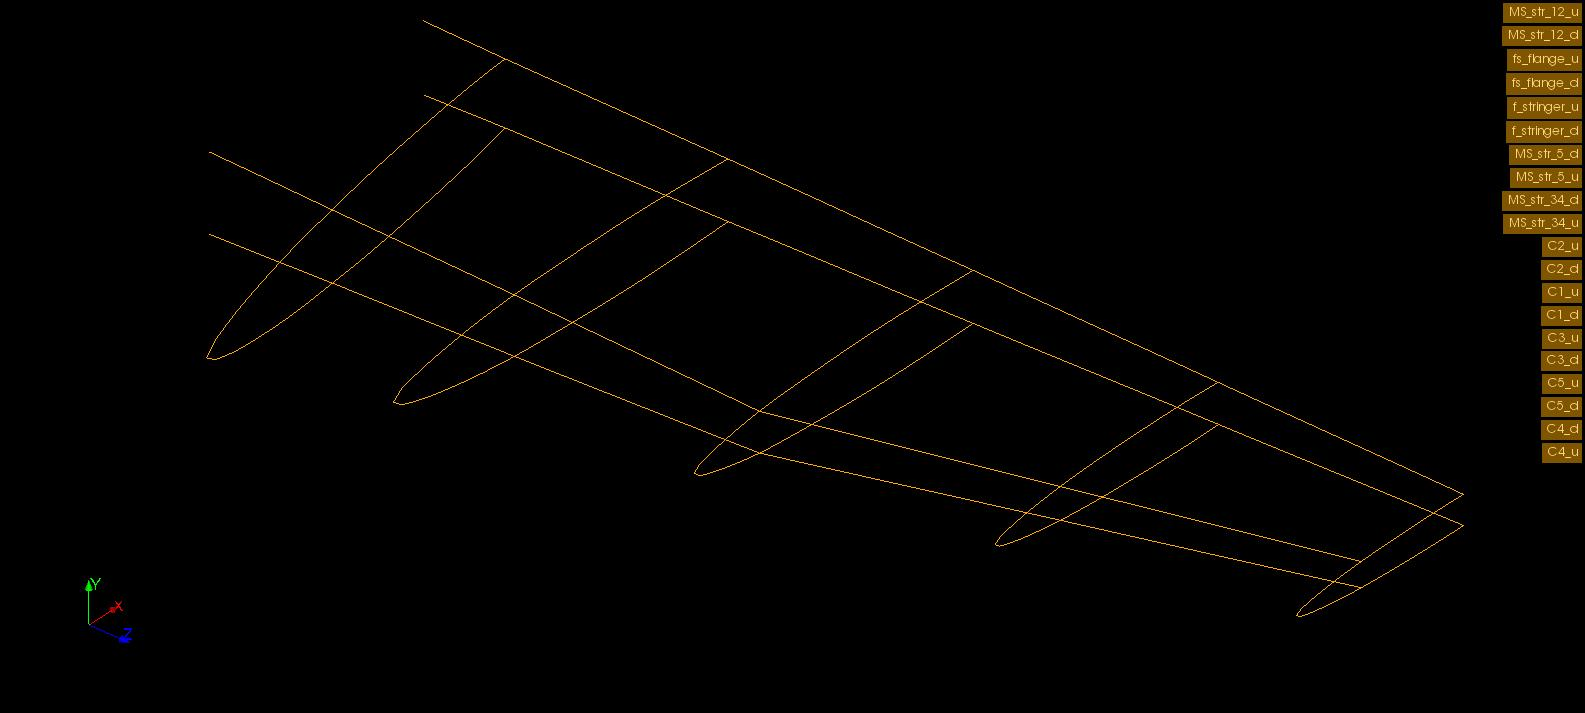
\includegraphics[width=.90\columnwidth]{mesh3.jpg}\label{fig:mesh3}} \\
	\caption[Mesh Stabilizzatore SF260]{mesh dello stabilizzatore} % The text in the square bracket is the caption for the list of figures while the text in the curly brackets is the figure caption
	\label{fig:mesh}
\end{figure}


\newpage


\section{Analisi Preliminari}

Prima con procedere alle analisi con i carichi dovuti a raffica e manovra, si è deciso di eseguire dei test preliminari con carichi semplificati, in modo da poter eseguire un confronto con un modello analitico a semiguscio e verificare così la validità del modello finora realizzato. Per quanto riguarda i vincoli sono state adottate le condizioni descritte in \ref{sec:vincoli}.\\
Sono stati eseguiti due test:

\begin{itemize}
	\item Momento torcente $M_z = 1000 N \cdot mm$ applicato alla centina 5 tramite un elemento di tipo \emph{RBE3}	
	\item Momento flettente $M_x = 1000 N \cdot mm$ applicato alla centina 5 tramite un elemento di tipo \emph{RBE3}
\end{itemize}

Sono stati poi misurati gli spostamenti medi e le rotazioni medie della centina 5 e confrontati con i risultati analitici.

\subsection{Simulazione momento torcente}

La simulazione fornisce un valore medio di rotazione intorno a \emph{z} pari a $3.104\cdot 10^{-5} rad$.

La figura \ref{fig:Mztest} mostra l'andamento della deformazione.

\begin{figure}[htb]
	\centering 
	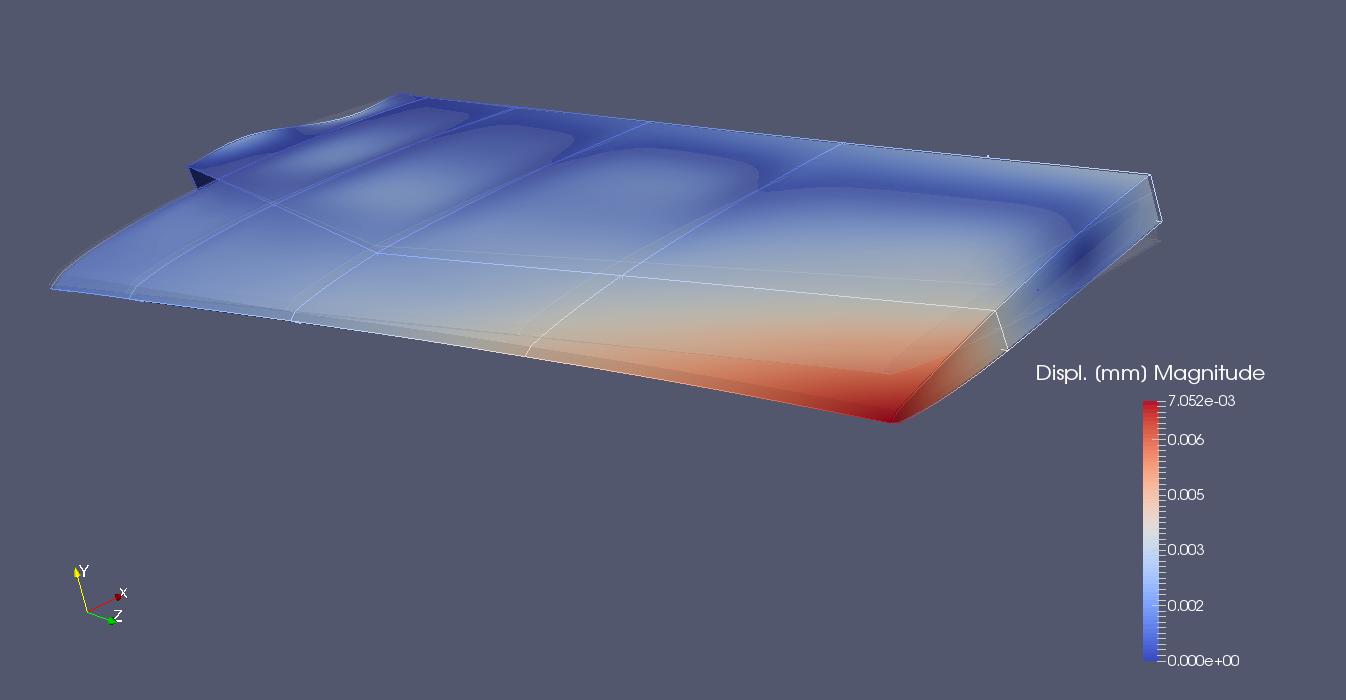
\includegraphics[width=0.9\columnwidth]{Mz_test.png} 
	\caption[Test Mz]{Test momento torcente} % The text in the square bracket is the caption for the list of figures while the text in the curly brackets is the figure caption
	\label{fig:Mztest} 
\end{figure}



\subsection{Simulazione momento flettente}

La simulazione fornisce un valore medio di rotazione intorno a \emph{x} pari a $1.548\cdot 10^{-5} rad$ ed uno spostamento medio lungo \emph{y} di $-1.01 \cdot 10^{-2}mm$.

La figura \ref{fig:Mxtest} mostra l'andamento della deformazione.

\begin{figure}[htb]
	\centering 
	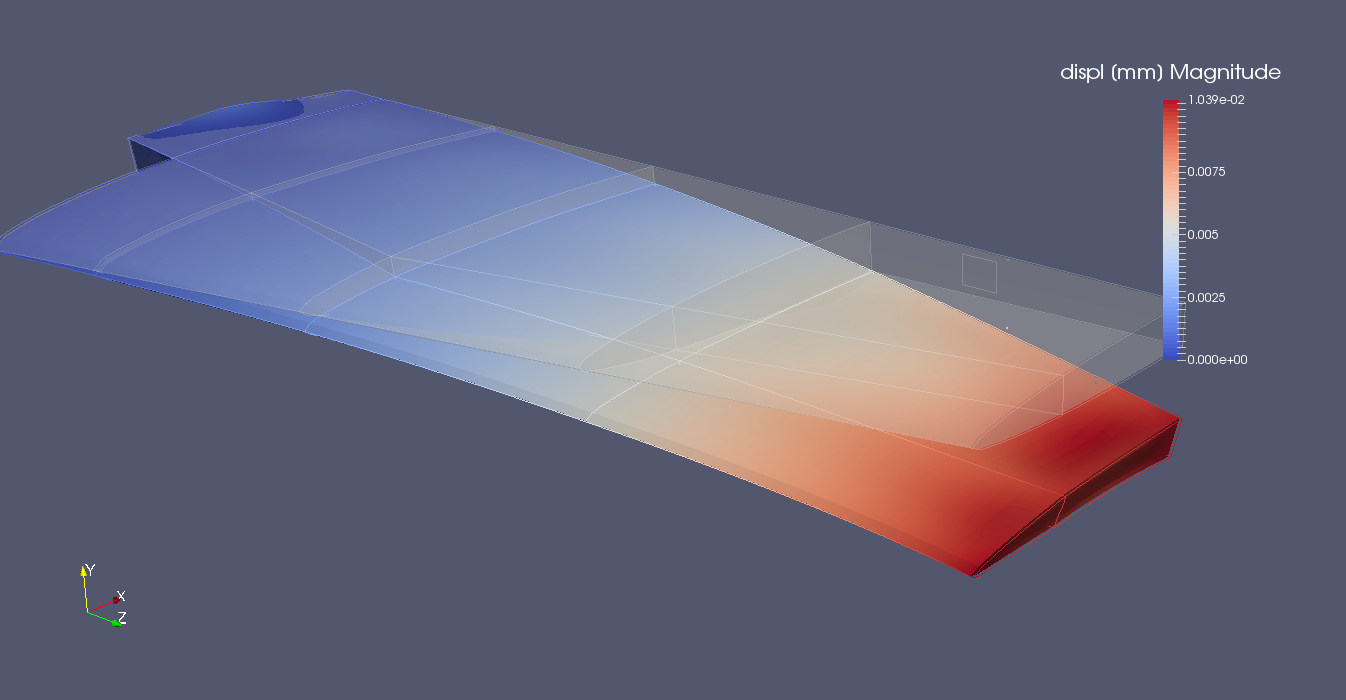
\includegraphics[width=0.9\columnwidth]{Mx_test.png} 
	\caption[Test Mx]{Test momento flettente} % The text in the square bracket is the caption for the list of figures while the text in the curly brackets is the figure caption
	\label{fig:Mxtest} 
\end{figure}


\section{Calcolo tramite teoria a semiguscio}

Per il corso di \emph{Strutture Aerospaziali} avevo sviluppato un programma per il calcolo dei parametri delle sezioni a semiguscio. Il codice è disponibile qui: \url{https://github.com/Ccaccia73/semimonocoque}. In particolare, i calcoli sono riportati qui: \url{http://nbviewer.jupyter.org/github/ccaccia73/semimonocoque/blob/master/10_Stab_SF260.ipynb} .

\subsection{Modello a semiguscio}

Lo stabilizzatore è stato suddiviso in 5 sezioni. Come larghezza è stata considerato il valore medio del tratto in esame. Si è trascurato l'angolo di inclinazione della centina 1 e sono state considerate le aree e gli spessori determinati in precedenza. Per i longheroni si è utilizzato il metodo dell'\emph{area collaborante}.

La figura \ref{fig:semiguscio} illustra le 5 sezioni descritte nel modello a semiguscio. I valori dei parametri sono visibili al link sopra.


\begin{figure}[tb]
	\centering
	\subfloat[Sezione 1]{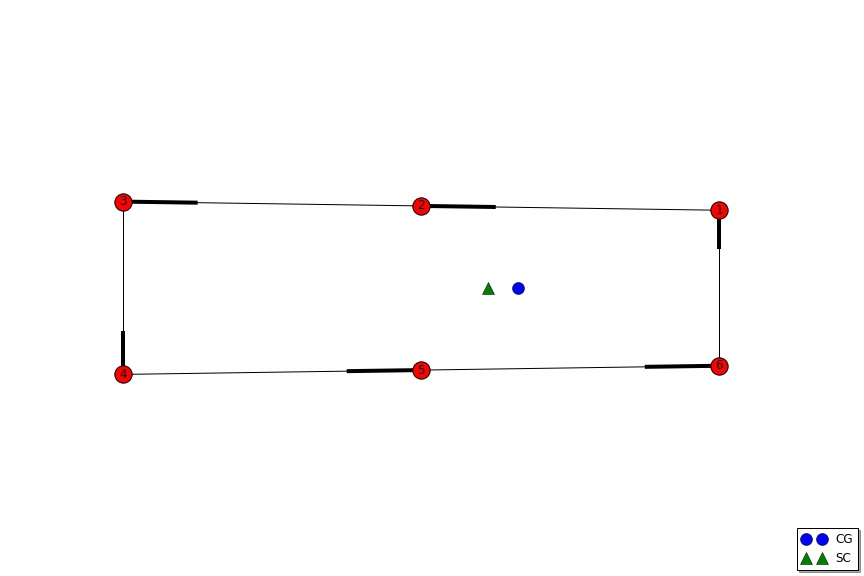
\includegraphics[width=.45\columnwidth]{sect1.jpg}} \quad
	\subfloat[Sezione 2]{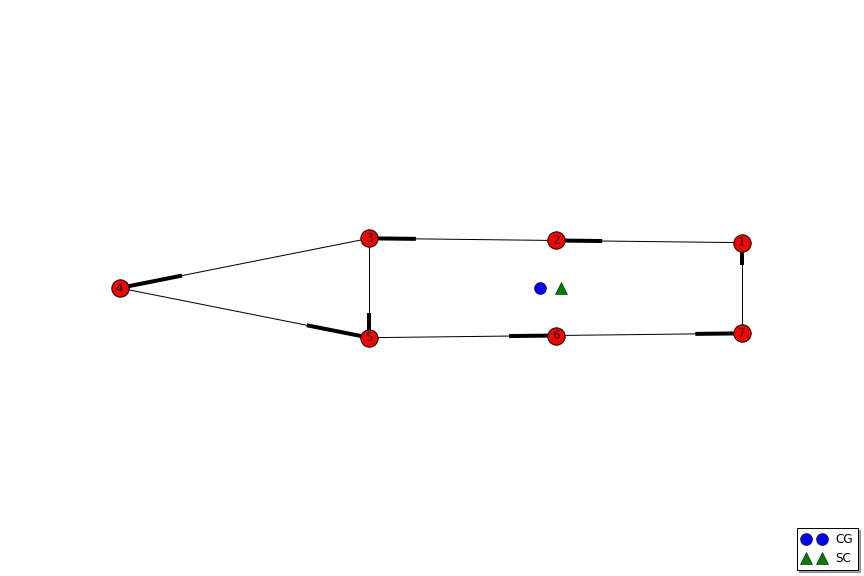
\includegraphics[width=.45\columnwidth]{sect2.jpg}} \\
	\subfloat[Sezione 3]{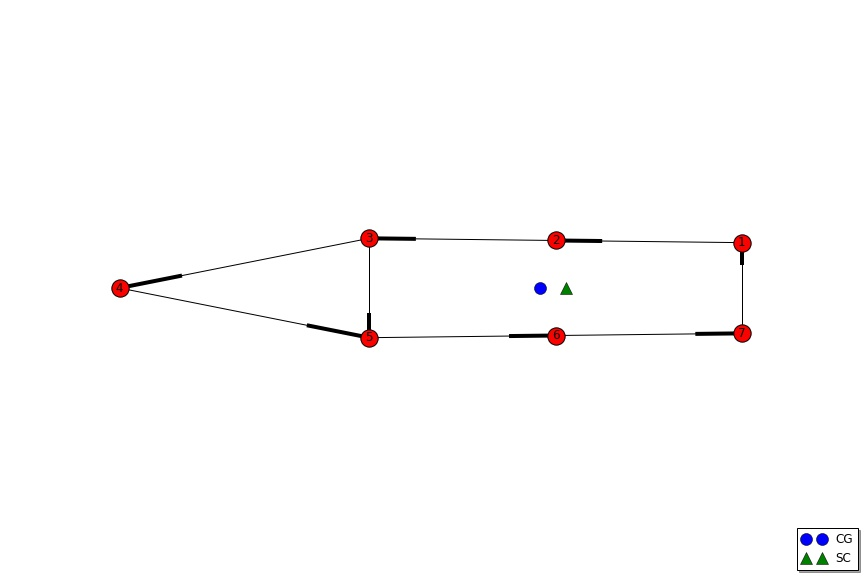
\includegraphics[width=.45\columnwidth]{sect3.jpg}} \quad
	\subfloat[Sezione 4]{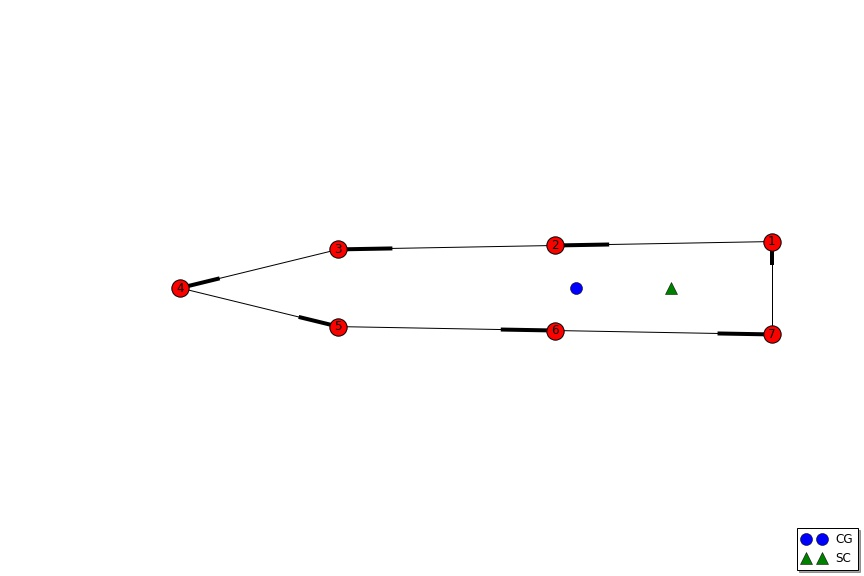
\includegraphics[width=.45\columnwidth]{sect4.jpg}} \\
	\subfloat[Sezione 5]{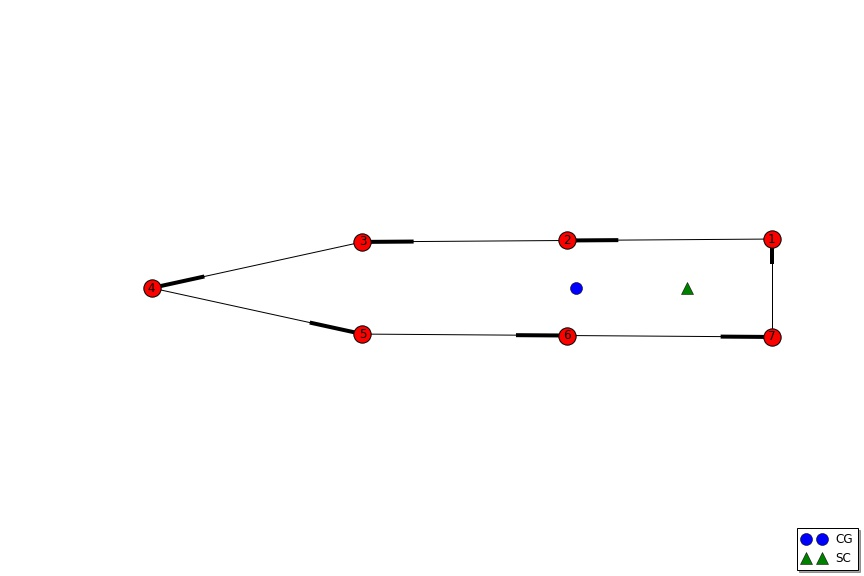
\includegraphics[width=.45\columnwidth]{sect5.jpg}} \\
	\caption[descrizione a semiguscio]{Sezioni a semiguscio dello stabilizzatore} % The text in the square bracket is the caption for the list of figures while the text in the curly brackets is the figure caption
	\label{fig:semiguscio}
\end{figure}


\subsection{Calcolo sezione sottoposta momento torcente}

Il modello a semiguscio fornisce una stima della rigidezza torsionale $J_{ti}$ per ogni tratto dello stabilizzatore. L'angolo totale di torsione viene calcolato tramite:

\begin{equation}
	\phi = \frac{M_z}{G} \cdot \sum_{i=1}^{5} \frac{L_i}{J_{ti}}
	\label{eq:sg_torque}
\end{equation}

con $L_i$ lunghezza del tratto i-esimo.\\
Il calcolo fornisce un valore di $\phi = 3.021 \cdot 10^{-5}$ rad.



\subsection{Calcolo sezione sottoposta momento flettente}

Il modello a semiguscio fornisce una stima della rigidezza flessionale $J_{xi}$ per ogni tratto dello stabilizzatore. L'angolo di flessione all'estremità viene calcolato tramite:


\begin{equation}
\theta = \frac{M_x}{E} \cdot \sum_{i=1}^{5} \frac{L_i}{J_{xi}}
\label{eq:sg_tip_flex}
\end{equation}

Il calcolo fornisce un valore di $\theta = 1.688 \cdot 10^{-5}$ rad.

Lo spostamento verticale $\delta$ dell'estremità deriva dalle seguenti espressioni:

\begin{equation}
\delta = \int_{0}^{l}M_x \cdot \frac{z-l}{EJ_x(z)}dz
\label{eq:sg_tip1}
\end{equation}

Suddividendo l'integrale nei tratti a $J_x$ costante si ottiene:

\begin{equation}
\delta = \sum_{i=1}^{5} \frac{l_i}{EJ_{xi}} \left\{ \frac{\bar{z}_i}{2}  - l  \right\} 
\label{eq:sg_tip2}
\end{equation}

Con $l_i$ lunghezza del tratto i-esimo e $\bar{z}_i$ posizione di metà tratto.\\
Il calcolo fornisce un valore di $\delta = -0.0085mm$.


\subsection{Confronto dei risultati:}

\begin{table}[hbt]
	\caption{Confronto risultati}
	\centering
	\begin{tabular}{lcc}
		\toprule
		& \multicolumn{2}{c}{Valori} \\
		\cmidrule(r){2-3}
		 & SG & FEM \\
		\midrule
		tors. $\phi \ [\mu rad]$ & $30.21$ & $31.04$ \\
		flex. $\theta \ [\mu rad]$ & $16.88$ & $15.48$ \\
		flex. $\delta \ [\mu m]$ & $-85$ & $-101$ \\
		\bottomrule
	\end{tabular}
	\label{tab:comp}
\end{table}

La rispondenza tra il modello ad elementi finiti ed il modello a semiguscio viene ritenuta buona, pertanto si considera il modello \emph{FEM} affidabile.

\newpage


\section{Vincoli}
\label{sec:vincoli}




\section{Carichi}

\subsection{Carichi sulle centine}


\subsection{Carichi sui longheroni}



\section{Analisi}

\newpage


\paragraph{Paragraph Description} \lipsum[7] % Dummy text

\paragraph{Different Paragraph Description} \lipsum[8] % Dummy text

%------------------------------------------------

\subsection{Math}

\lipsum[4] % Dummy text

\begin{equation}
\cos^3 \theta =\frac{1}{4}\cos\theta+\frac{3}{4}\cos 3\theta
\label{eq:refname2}
\end{equation}

\lipsum[5] % Dummy text

\begin{definition}[Gauss] 
To a mathematician it is obvious that
$\int_{-\infty}^{+\infty}
e^{-x^2}\,dx=\sqrt{\pi}$. 
\end{definition} 

\begin{theorem}[Pythagoras]
The square of the hypotenuse (the side opposite the right angle) is equal to the sum of the squares of the other two sides.
\end{theorem}

\begin{proof} 
We have that $\log(1)^2 = 2\log(1)$.
But we also have that $\log(-1)^2=\log(1)=0$.
Then $2\log(-1)=0$, from which the proof.
\end{proof}

%----------------------------------------------------------------------------------------
%	RESULTS AND DISCUSSION
%----------------------------------------------------------------------------------------

\section{Results and Discussion}

\lipsum[10] % Dummy text

%------------------------------------------------

\subsection{Subsection}

\lipsum[11] % Dummy text

\subsubsection{Subsubsection}

\lipsum[12] % Dummy text

\begin{description}
\item[Word] Definition
\item[Concept] Explanation
\item[Idea] Text
\end{description}

\lipsum[12] % Dummy text

\begin{itemize}[noitemsep] % [noitemsep] removes whitespace between the items for a compact look
\item First item in a list
\item Second item in a list
\item Third item in a list
\end{itemize}

\subsubsection{Table}

\lipsum[13] % Dummy text

\begin{table}[hbt]
\caption{Table of Grades}
\centering
\begin{tabular}{llr}
\toprule
\multicolumn{2}{c}{Name} \\
\cmidrule(r){1-2}
First name & Last Name & Grade \\
\midrule
John & Doe & $7.5$ \\
Richard & Miles & $2$ \\
\bottomrule
\end{tabular}
\label{tab:label}
\end{table}

Reference to Table~\vref{tab:label}. % The \vref command specifies the location of the reference

%------------------------------------------------


%----------------------------------------------------------------------------------------
%	BIBLIOGRAPHY
%----------------------------------------------------------------------------------------

%\renewcommand{\refname}{\spacedlowsmallcaps{References}} % For modifying the bibliography heading

%\bibliographystyle{unsrt}

%\bibliography{sample.bib} % The file containing the bibliography

%----------------------------------------------------------------------------------------

\end{document}